\documentclass{lab_sheet}
\usepackage{nccmath}
\usepackage{tikz}
\usetikzlibrary{arrows}
\usepackage{hyperref}
\newcommand\ddfrac[2]{\frac{\displaystyle #1}{\displaystyle #2}}
\newcommand{\proteusObservationA}[4]{ 
\begin{figure}[H]
   \begin{minipage}[b]{0.60\linewidth}
     \centering
     \includegraphics[width=\linewidth]{../Figures/#1.PDF}
   \end{minipage}%
   \begin{minipage}[b]{0.40\linewidth}
     \centering
 \begin{tabular}[b]{|M{4cm}|M{1cm}|}
   \hline
   \multicolumn{2}{|c|}{Noted Values} \\
   \hline \hline
   DC gain (in dB) & #2\\ \hline
   Half power frequency (in KHz) & #3\\ \hline
 \end{tabular}
 \end{minipage}
 \caption{Observation for #4}
 \label{fig:prot_obs_a_#1}
 \end{figure}
}
\newcommand{\figquestion}{
    \begin{circuitikz}[american]   
    \draw
    (0,0) node [op amp, noinv input up] (opamp) {}
    (-7,0.5) node [left] {$V_{1}$} to [R, l=$R_1$, o-*] (-5,0.5) node[label={[font=\footnotesize]north west:$b$}] {} node[label={[font=\footnotesize]below:$V_b$}] {} to [R, l=$R_2$] (-3,0.5) to [short](opamp.+) 
    (-5,0.5) to [short] (-5,1.5) to [C,l=$C_1$] (1,1.5)-| (opamp.out) to [short,*-o] (2,0) node [right] {$V_{2}$}
    (-3,0.5) node[label={[font=\footnotesize]above:$a$}] {} node[label={[font=\footnotesize]south east:$V_a$}] {} to [C,l=$C_2$,*-] (-3,-1.5) node[ground]{}
    (opamp.-) |- (-1,-1.5) to [R,l=$R_b$] (1,-1.5)-| (opamp.out) 
    (-1.2, -1.5) to [R,l=$R_a$, *-] (-1.2,-3.5) node[ground]{}
    ;
        \end{circuitikz}
}
\newcommand{\figeqv}{
    \begin{circuitikz}[american]   
        \draw
      (0,0) node [left] {$V_{1}$} to [R,l=$R_1$,o-o] (2,0)
      (4.5,0) node [left] {$V_{1}$} to [R,l=$R_x$,o-] (6.5,0) to [R,l=$R_y$,*-] (6.5,-2) node[ground]{}
      (6.5,0) to [short,-o] (7,0)
        ;
        \draw[->,thick](2.5,0) -- (3.5,0);
            \end{circuitikz}
}

\newcommand{\figeqvi}{
    \begin{circuitikz}[american]   
        \draw
      (0,0) node [left] {$V_{1}$} to [R,l=$R_1'$,o-o] (2,0)
      (4.5,0) node [left] {$V_{1}$} to [R,l=$R_x'$,o-] (6.5,0) to [R,l=$R_y'$,*-] (6.5,-2) node[ground]{}
      (6.5,0) to [short,-o] (7,0)
        ;
        \draw[->,thick](2.5,0) -- (3.5,0);
            \end{circuitikz}
}

\newcommand{\figgain}{
    \begin{circuitikz}[american]   
        \draw
        (0,0) node [op amp, noinv input up] (opamp) {}
        (-7,0.5) node [left] {$V_{1}$} to [R, l=$R_x$, o-*] (-5,0.5) to [R, l=$R_2$] (-3,0.5) to [short](opamp.+) 
        (-5,0.5) to [short] (-5,1.5) to [C,l=$C_1$] (1,1.5)-| (opamp.out) to [short,*-o] (2,0) node [right] {$V_{2}$}
        (-3,0.5) to [C,l=$C_2$,*-] (-3,-1.5) node[ground]{}
        (opamp.-) |- (-1,-1.5) to [R,l=$R_b$] (1,-1.5)-| (opamp.out) 
        (-1.2, -1.5) to [R,l=$R_a$, *-] (-1.2,-3.5) node[ground]{}
        (-5,0.5) to [R, l=$R_y$] (-5,-1.5) node[ground]{}
        ;
            \end{circuitikz}
}

\newcommand{\figfourthorder}{
    \begin{circuitikz}[american, scale = 0.97, transform shape]
        \draw
        (0,0) node [op amp, noinv input up] (opamp) {}
        (7,-0.5) node [op amp, noinv input up] (op) {}
        (-6,0.5) node [left] {$V_{1}$} to [R, l=\footnotesize$2.2351\text{ }\Omega$, o-*] (-4,0.5) to [R, l=\footnotesize$1\text{ }\Omega$] (-2,0.5) to [short](opamp.+) 
        (-4,0.5) to [short] (-4,1.5) to [C,l=\footnotesize$1\text{ F}$] (0,1.5)-| (opamp.out) to [R,*-*,l=\footnotesize$1.1522 \text{ }\Omega$] (3,0) to [R, l=\footnotesize$1\text{ }\Omega$] (5,0) to [short](op.+)
        (3,0) to [short] (3,1) to [C,l=\footnotesize$1 \text{ F}$] (7,1)-| (op.out) to [short,*-o] (8.5,-0.5) node [right] {$V_{2}$}
        (5,0) to [C,l_=\footnotesize$1 \text{ F}$] (5,-2)node[ground]{}
        (-2,0.5) to [C,l_=\footnotesize$1 \text{ F}$,*-] (-2,-1.5) node[ground]{}
        (opamp.-) |- (-1,-1.5) to [R,l_=\footnotesize$1.2347 \text{ }\Omega$] (1,-1.5)-| (opamp.out) 
        (-1.2, -1.5) to [R,l_=\footnotesize$1 \text{ }\Omega$, *-] (-1.2,-3.5) node[ground]{}
        (op.-) |- (6,-2) to [R,l_=\footnotesize$0.1522 \text{ }\Omega$] (8,-2)-| (op.out) 
        (5.8, -2) to [R,l_=\footnotesize$1 \text{ }\Omega$, *-] (5.8,-4) node[ground]{}
        (-4,0.5) to [R, l_=\footnotesize$1.8095\text{ }\Omega$] (-4,-1.5) node[ground]{}
        (3,0) to [R, l_=\footnotesize$7.57 \text{ }\Omega$] (3,-2) node[ground]{}
        ;
            \end{circuitikz}
}

\newcommand{\figfourthorderfinal}{
    \begin{circuitikz}[american, scale = 0.97, transform shape]
        \draw
        (0,0) node [op amp, noinv input up] (opamp) {}
        (7,-0.5) node [op amp, noinv input up] (op) {}
        (-6,0.5) node [left] {$V_{1}$} to [R, l=\footnotesize $2.2351\text{ K}\Omega$, o-*] (-4,0.5) to [R, l=\footnotesize$1\text{ K}\Omega$] (-2,0.5) to [short](opamp.+) 
        (-4,0.5) to [short] (-4,1.5) to [C,l=\footnotesize$50\text{ nF}$] (0,1.5)-| (opamp.out) to [R,*-*,l=\footnotesize$1.1522 \text{ K}\Omega$] (3,0) to [R, l=\footnotesize$1\text{ K}\Omega$] (5,0) to [short](op.+)
        (3,0) to [short] (3,1) to [C,l=\footnotesize$50 \text{ nF}$] (7,1)-| (op.out) to [short,*-o] (8.5,-0.5) node [right] {$V_{2}$}
        (5,0) to [C,l_=\footnotesize$50 \text{ nF}$] (5,-2)node[ground]{}
        (-2,0.5) to [C,l_=\footnotesize$50 \text{ nF}$,*-] (-2,-1.5) node[ground]{}
        (opamp.-) |- (-1,-1.5) to [R,l_=\footnotesize$1.2347 \text{ K}\Omega$] (1,-1.5)-| (opamp.out) 
        (-1.2, -1.5) to [R,l_=\footnotesize$1 \text{ K}\Omega$, *-] (-1.2,-3.5) node[ground]{}
        (op.-) |- (6,-2) to [R,l_=\footnotesize$152.2 \text{ }\Omega$] (8,-2)-| (op.out) 
        (5.8, -2) to [R,l_=\footnotesize$1 \text{ K}\Omega$, *-] (5.8,-4) node[ground]{}
        (-4,0.5) to [R, l_=\footnotesize$1.8095\text{ K}\Omega$] (-4,-1.5) node[ground]{}
        (3,0) to [R, l_=\footnotesize$7.57 \text{ K}\Omega$] (3,-2) node[ground]{}
        ;
            \end{circuitikz}
}

\newcommand{\figfourthorderhp}{
    \begin{circuitikz}[american, scale = 0.97, transform shape]
        \draw
        (0,0) node [op amp, noinv input up] (opamp) {}
        (7,-0.5) node [op amp, noinv input up] (op) {}
        (-6,0.5) node [left] {$V_{1}$} to [C, l=\footnotesize$0.4474\text{ F}$, o-*] (-4,0.5) to [C, l=\footnotesize$1\text{ F}$] (-2,0.5) to [short](opamp.+) 
        (-4,0.5) to [short] (-4,1.5) to [R,l=\footnotesize$1\text{ } \Omega$] (0,1.5)-| (opamp.out) to [C,*-*,l=\footnotesize$0.8679 \text{ F}$] (3,0) to [C, l=\footnotesize$1\text{ F}$] (5,0) to [short](op.+)
        (3,0) to [short] (3,1) to [R,l=\footnotesize$1 \text{ }\Omega$] (7,1)-| (op.out) to [short,*-o] (8.5,-0.5) node [right] {$V_{2}$}
        (5,0) to [R,l_=\footnotesize$1 \text{ }\Omega$] (5,-2)node[ground]{}
        (-2,0.5) to [R,l_=\footnotesize$1 \text{ }\Omega$,*-] (-2,-1.5) node[ground]{}
        (opamp.-) |- (-1,-1.5) to [R,l_=\footnotesize$1.2347 \text{ }\Omega$] (1,-1.5)-| (opamp.out) 
        (-1.2, -1.5) to [R,l_=\footnotesize$1 \text{ }\Omega$, *-] (-1.2,-3.5) node[ground]{}
        (op.-) |- (6,-2) to [R,l_=\footnotesize$0.1522 \text{ }\Omega$] (8,-2)-| (op.out) 
        (5.8, -2) to [R,l_=\footnotesize$1 \text{ }\Omega$, *-] (5.8,-4) node[ground]{}
        (-4,0.5) to [C, l_=\footnotesize$0.5526\text{ F}$] (-4,-1.5) node[ground]{}
        (3,0) to [C, l_=\footnotesize$0.1321 \text{ F}$] (3,-2) node[ground]{}
        ;
            \end{circuitikz}
}

\newcommand{\figfourthorderhpfinal}{
    \begin{circuitikz}[american, scale = 0.97, transform shape]
        \draw
        (0,0) node [op amp, noinv input up] (opamp) {}
        (7,-0.5) node [op amp, noinv input up] (op) {}
        (-6,0.5) node [left] {$V_{1}$} to [C, l=\footnotesize$14.913\text{ nF}$, o-*] (-4,0.5) to [C, l=\footnotesize$33.33\text{ nF}$] (-2,0.5) to [short](opamp.+) 
        (-4,0.5) to [short] (-4,1.5) to [R,l=\footnotesize$1\text{ K} \Omega$] (0,1.5)-| (opamp.out) to [C,*-*,l=\footnotesize$28.93\text{ nF}$] (3,0) to [C, l=\footnotesize$33.33\text{ nF}$] (5,0) to [short](op.+)
        (3,0) to [short] (3,1) to [R,l=\footnotesize$1 \text{ K}\Omega$] (7,1)-| (op.out) to [short,*-o] (8.5,-0.5) node [right] {$V_{2}$}
        (5,0) to [R,l_=\footnotesize$1 \text{ K}\Omega$] (5,-2)node[ground]{}
        (-2,0.5) to [R,l_=\footnotesize$1 \text{ K}\Omega$,*-] (-2,-1.5) node[ground]{}
        (opamp.-) |- (-1,-1.5) to [R,l_=\footnotesize$1.2347 \text{ K}\Omega$] (1,-1.5)-| (opamp.out) 
        (-1.2, -1.5) to [R,l_=\footnotesize$1 \text{ K}\Omega$, *-] (-1.2,-3.5) node[ground]{}
        (op.-) |- (6,-2) to [R,l_=\footnotesize$152.2 \text{ }\Omega$] (8,-2)-| (op.out) 
        (5.8, -2) to [R,l_=\footnotesize$1 \text{ K}\Omega$, *-] (5.8,-4) node[ground]{}
        (-4,0.5) to [C, l_=\footnotesize$18.42\text{ nF}$] (-4,-1.5) node[ground]{}
        (3,0) to [C, l_=\footnotesize$4.4\text{ nF}$] (3,-2) node[ground]{}
        ;
            \end{circuitikz}
}

\begin{document}
    \titlePage{Design of Higher Order Active Filter using Sallen and Key Biquad Circuit}{July 28, 2021}
    \pagenumbering{roman}
    \clearpage
    \tableofcontents
    \clearpage
    \phantomsection
    \addcontentsline{toc}{section}{\bfseries{List of Figures}}
    \listoffigures
    \phantomsection
    \addcontentsline{toc}{section}{\bfseries{List of Tables}}
    \listoftables
    \clearpage
    \pagenumbering{arabic}
    \section{Objectives}
    \begin{itemize}
        \item To be familiar with the design of higher order active filters using cascaded biquad.
        \item To be familiar with design of filter using Sallen and Key biquad circuit.
        \item To be familiar with RC-CR transformation.
    \end{itemize}
    \section{Exercises}
    \mysub{Desgin of higher order active filters}
    \problem{What are the different techniques to design higher order active filters? Explain.}
    Higher order active filters are a necessary part of telecommunication and instrumentation systems to satisfy the need of selectivity. The design of higher order active filters can be performed by two methods,
    \begin{enumerate}
        \item Cascade of biquad circuits
        \item Active simulation of passive filters
        \begin{enumerate}
            \item Elemental simulation
            \begin{itemize}
                \item Ladder design with simulated inductors
                \item Ladder design with Frequency-Dependent Negative Resistor (FDNR)
            \end{itemize}
            \item Functional simulation
            \begin{itemize}
                \item Leapfrog simulation of ladders
            \end{itemize}
        \end{enumerate}
    \end{enumerate}
    Since this lab experiment is based on the design of higher order active filters using cascade of biquad circuits, it is explained in detail. However, the active simulation of passive circuits is only introduced in this report.
    \subsubsection{Cascade of biqaud circuits}
    For a higher order active filter with transfer function $T(s)$, the realization is possible as the ratio of the output voltage to input voltage of a cascade connection of lower order stages that don't cause load effect. For this to be possible, the output impedance of each stage needs to be lower than the input impedance of the following stage at all interested frequencies.
    \begin{figure}[H]
        \centering
        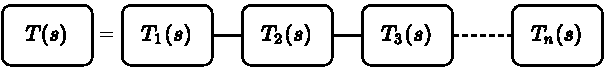
\includegraphics[width=\linewidth]{../Figures/cascade_block}
        \caption{Cascade of biquad circuits}
        \label{fig:cascade_block}
    \end{figure}
    While designing a circuit with transfer function $T(s)$ using biquadratic terms $T_i(s)$ in a cascaded system, we have the following degree of freedom,
    \begin{enumerate}
        \item Pole-zero pairing i.e. which pole with zero of $T(s)$ will be paired to form each $T_i(s)$.
        \item Physical position of each biquad in the cascade system.
        \item Distribution of the overall gain in the various biquad circuits.
    \end{enumerate}
    This method of designing higher order active filters is made possible due to the use of operational amplifiers in designs of active filters. Since op-amp offers high input impedance and low output impedance, loading effect is nullified, which we use as an advantage to cascade different stages of active filters to get the desired transfer function for a final filter circuit.\\
    If $T(s)$ is the required transfer function given as,
    \begin{equation*}
        T(s)=\frac{a_ms^m+a_{m-1}s^{m-1}+\cdots+a_0}{s^n+b_{n-1}s^{n-1}+\cdots+b_0}
    \end{equation*}
    For $n$ as even, $T(s)$ is expressed as,
    \begin{equation*} 
            T(s)=\prod_{i=1}^{\frac{n}{2}}\frac{a_{2i}s^2+a_{1i}s+a_{0i}}{s^2+b_{1i}s+b_{0i}}=\prod_{i=1}^{\frac{n}{2}}T_i(s)
    \end{equation*}
    For $n$ as odd, $T(s)$ is expressed as,
    \begin{equation*} 
      \begin{aligned}
          T(s)=\frac{a_{11}s+a_{01}}{s+b_{01}}\prod_{i=2}^{\frac{n-1}{2}}\frac{a_{2i}s^2+a_{1i}s+a_{0i}}{s^2+b_{1i}s+b_{0i}}=T_1(s)\prod_{i=2}^{\frac{n-1}{2}}T_i(s)
      \end{aligned}
\end{equation*}
    \subsubsection{Active simulation of passive filters}
    Since the design of higher order active filters are limited due to the value of inductance, a way to design higher order active filters is by simulating the inductance behavior in the circuit using elemental simulation. This can be done by using a Generalized Impedance Converter (GIC), a two port network that is used primarily to convert one form of impedance into another. A grounded inductor in a passive circuit is replaced with a GIC to convert the passive circuit into active. Another way of performing elemental simulation is by using a magnitude scaling factor of $K_m=\ddfrac{1}{s}$, which ultimately converts the resistor to a capacitor $\left(\ddfrac{R}{s}\right)$, an inductor to a resistor $(L)$, and the capacitor to a Frequency Dependent Negative Resistor (FDNR) $\left(\ddfrac{1}{s^2C}\right)$ which is also realized using a GIC.\\
    Similarly, functional simulation (leapfrog simulation) is another way to get active simulation of passive filters. Each component in the passive circuit is first replaced by their equivalent impedance or admittance and admittance or impedance groups are created based on same current (series) or same voltage (parallel) configuration giving rise to a block diagram equivalent to the original circuit. Each block is then implemented either by using an inverting summer (for summing blocks) or active circuits (for admittance and impedance blocks) to complete the active simulation of the passive filter.
    \mysub{Derivation of transfer function of Sallen-Key biquad circuit}
    \problem{From the circuit given in Figure~\ref{fig:ques} derive the transfer function $\ddfrac{V_2(s)}{V_1(s)}$.}
    \begin{figure}[H]
        \centering
        \figquestion
        \caption{Sallen-Key lowpass filter}
        \label{fig:ques}
    \end{figure}
    Let us consider the voltage at nodes $a$ and $b$ as $V_a$ and $V_b$ respectively. The circuit is in an non-inverting configuration, so the gain of the circuit has the following relationship,
    \begin{equation}
        \begin{aligned}[b]
            \frac{V_2}{V_a}&=\left(1+\frac{R_b}{R_a}\right)\\
            \therefore V_a&=\frac{V_2}{K}
        \end{aligned}
        \label{eqn:va-gain}
    \end{equation}
    where, $K=\left(1+\ddfrac{R_b}{R_a}\right)$ is the gain.\\
    Applying nodal analysis at node $a$, we get,
    \begin{equation}
        \begin{aligned}[b]
            &\Rightarrow \frac{V_a-V_b}{R_2}+\ddfrac{V_a}{\frac{1}{sC_2}}=0\\
            &\Rightarrow \frac{V_a}{R_2}-\frac{V_b}{R_2}+sV_aC_2=0\\
            &\Rightarrow V_a\left(\frac{1}{R_2}+sC_2\right)=\frac{V_b}{R_2}\\
            &\therefore V_b=V_aR_2\left(\frac{1}{R_2}+sC_2\right)
        \end{aligned}
        \label{eqn:node-a}
    \end{equation}

    Substituting the value for $V_a$ from Equation~\ref{eqn:va-gain} into Equation~\ref{eqn:node-a}, we get,
    \begin{equation}
        \begin{aligned}[b]
            &\Rightarrow V_b=\frac{V_2R_2}{K}\left(\frac{1}{R_2}+sC_2\right)\\
            & \therefore V_b = \frac{V_2}{K}\left(1+sC_2R_2\right)
        \end{aligned}
        \label{eqn:vb-v2}
    \end{equation}
    

    Applying nodal analysis at node $b$, we get,
    \begin{equation}
        \begin{aligned}[b]
            &\Rightarrow \frac{V_b-V_a}{R_2}+\frac{V_b-V_1}{R_1}+\ddfrac{V_b-V_2}{\frac{1}{sC_1}}=0\\
            &\therefore V_b \left(\frac{1}{R_2}+\frac{1}{R_1}+sC_1\right)-\frac{V_a}{R_2}=\frac{V_1}{R_1}+sV_2C_1
        \end{aligned}
        \label{eqn:node-b}
    \end{equation}

    Substituting the values for $V_a$ and $V_b$ from Equation~\ref{eqn:va-gain} and Equation~\ref{eqn:vb-v2} into Equation~\ref{eqn:node-b}, we get,
    \begin{equation}
        \begin{aligned}[b]
            &\Rightarrow \frac{V_2}{K}\left(1+sC_2R_2\right) \left(\frac{1}{R_2}+\frac{1}{R_1}+sC_1\right)-\frac{V_2}{KR_2}=\frac{V_1}{R_1}+sV_2C_1\\
            &\Rightarrow \frac{V_2}{K}\left(1+sC_2R_2\right) \left(\frac{R_1+R_2+sC_1R_1R_2}{R_1R_2}\right)-\frac{V_2}{KR_2}-sV_2C_1=\frac{V_1}{R_1}\\
            &\Rightarrow \frac{V_2\left[\left(1+sC_2R_2\right)\left(R_1+R_2+sC_1R_1R_2\right)-R_1-sKC_1R_1R_2\right]}{KR_1R_2}=\frac{V_1}{R_1}\\
            &\Rightarrow \frac{V_2}{V_1}=\frac{KR_2}{R_2+sC_1R_1R_2+sC_2R_1R_2+sC_2R_2^2+s^2C_1C_2R_1R_2^2-sKC_1R_1R_2}\\
            &\Rightarrow \frac{V_2}{V_1}=\frac{KR_2}{s^2C_1C_2R_1R_2^2+s\left(C_1R_1R_2+C_2R_1R_2+C_2R_2^2-KC_1R_1R_2\right)+R_2}\\
            &\Rightarrow \frac{V_2}{V_1}=\ddfrac{\frac{KR_2}{C_1C_2R_1R_2^2}}{s^2+s\left(\frac{C_1R_1R_2+C_2R_1R_2+C_2R_2^2-KC_1R_1R_2}{C_1C_2R_1R_2^2}\right)+\frac{R_2}{C_1C_2R_1R_2^2}}\\
            &\therefore T_{LP}(s)= \frac{V_2}{V_1}=\ddfrac{K\frac{1}{C_1C_2R_1R_2}}{s^2+s\left(\frac{1}{C_1R_1}+\frac{1}{C_1R_2}+\frac{1}{C_2R_2}-\frac{K}{C_2R_2}\right)+\frac{1}{C_1C_2R_1R_2}}
        \end{aligned}
        \label{eqn:tfr-final}
    \end{equation}

    \mysub{Design of fourth order butterworth filter}
    \problem{Realize the fourth order Butterworth filter (refer Table \ref{tbl:pole_location}) using Sallen-Key circuit. Perform gain compensation if necessary.}
    \begin{table}[H]
        \centering
        \begin{tabular}{|M{3cm}|M{3cm}|M{3cm}|M{3cm}|}
            \hline
            $n=2$ & $n=3$ & $n=4$ & $n=5$ \\
            \hline \hline
           $-0.7071068\pm j0.7071068$     & $-0.50\pm j 0.86603$ & $-0.3826834\pm j0.9238795$  & $-0.809017\pm j 0.5877852$  \\
           \hline
            ~       & $-1.0$  & $-0.9238795\pm j0.3826834$  & $-0.309017\pm j0.9510565$    \\
            \hline
            ~       & ~       & ~       & $-1.0$    \\
            \hline
            \end{tabular}
            \caption{Pole location for butterworth response}
            \label{tbl:pole_location}
    \end{table}
For a lowpass filter with poles at $s=-\alpha\pm j\beta$ and $s=-\alpha'\pm j\beta'$ the denominator polynomial is calculated as,
\begin{equation*}
    \begin{aligned}
        f_{den}(s)&=(s+\alpha+j\beta)(s+\alpha-j\beta)(s+\alpha'+j\beta')(s+\alpha'-j\beta') \\
        &=\left((s+\alpha)^2-j^2\beta^2\right)\left((s+\alpha')^2-j^2\beta'^2\right) \\
        &=\left(s^2+2\alpha s +\alpha^2+\beta^2\right)\left(s^2+2\alpha' s +\alpha'^2+\beta'^2\right)
    \end{aligned}
\end{equation*}
For given pole locations at $s=-0.3826834\pm j0.9238795$ and $s=-0.9238795\pm j0.3826834$, i.e. $\alpha=-0.3826834$, $\beta=0.9238795$, $\alpha'=-0.9238795$, $\beta'=0.3826834$ the denominator function is,
\begin{equation}
        f_{den}(s)=(s^2+0.7653s+1)(s^2+1.8478s+1)
        \label{eqn:den-derived}
 \end{equation}
 The denominator function for a general 2\textsuperscript{nd} order lowpass filter can be written as,
 \begin{equation}
     f_{den}^{g}(s)=s^2+s\left(\frac{\omega_o}{Q}\right)+\omega_o^2
     \label{eqn:den-general}
 \end{equation}
 We need to cascade two such 2\textsuperscript{nd} order lowpass filters to get the desired form of denominator equation as,
 \begin{equation}
    f_{den}^{c}(s)=\left(s^2+s\left(\frac{\omega_o}{Q}\right)+\omega_o^2\right)\left(s^2+s\left(\frac{\omega_o'}{Q'}\right)+\omega_o'^2\right)
    \label{eqn:den-cascaded}
\end{equation}
Comparing Equation~\ref{eqn:den-derived} and Equation~\ref{eqn:den-cascaded}, we get,
\begin{equation*}
    \begin{aligned}
        &\omega_o^2=1\Rightarrow\omega_o=\sqrt{1}=1 \text{ rad/s}\\
        &\frac{\omega_o}{Q}=0.7653\Rightarrow Q=\frac{\omega_o}{0.7653}=\frac{1}{0.7653}=1.3067\\
        &\omega_o'^2=1\Rightarrow\omega_o'=\sqrt{1}=1\text{ rad/s}\\
        &\frac{\omega_o'}{Q'}=1.8478\Rightarrow Q'=\frac{\omega_o'}{1.8478}=\frac{1}{1.8478}=0.5412\\
    \end{aligned}
\end{equation*}
Hence the filter parameters for the two stages of filters are, $\omega_o=1$, $Q=1.3067$, $H=1$, $\omega_o'=1$, $Q'=0.5412$, $H'=1$.
\subsubsection*{Stage I}
Let us design the first stage with the parameters $\omega_o=1$ rad/s, $Q=1.3067$ and $H=1$ using the default (equal element values) technique with elemental values $C_1=C_2=1\text{ F}$ and $R_1=R_2=R$ as,
\begin{equation*}
    \begin{aligned}
        &R=\frac{1}{\omega_o}\Rightarrow R=\frac{1}{1}=1 \text{ }\Omega\\
        & K=3-\frac{1}{Q}\Rightarrow K= 3-\frac{1}{1.3067}=2.2347
    \end{aligned}
\end{equation*}
We have, the relation for gain,
\begin{equation*}
    \begin{aligned}
        &K=1+\frac{R_b}{R_a}\Rightarrow \frac{R_b}{R_a}=K-1=2.2347-1=1.2347
    \end{aligned}
\end{equation*}
For $R_a=1\text{ }\Omega$, $R_b=1.2347\text{ }\Omega$. Since the calculated gain is $K=2.2347$, but we require a gain of $H=1$, we need to perform gain compensation, i.e. reduction in this case. For gain reduction, we have to replace $R_1$ in Figure~\ref{fig:ques} with an equivalent parallel circuit as,
\begin{figure}[H]
    \centering
    \figeqv
    \caption{$R_1=R_x||R_y$ equivalence circuit}
    \label{fig:eqv}
\end{figure}
From Figure~\ref{fig:eqv}, we have,
\begin{equation}
    \begin{aligned}[b]
       &R_1=R_x||R_y\\
       &\Rightarrow R_1=\frac{R_xR_y}{R_x+R_y}\\
       &\Rightarrow R_x+R_y=R_xR_y
    \end{aligned}
    \label{eqn:ry-rx-parallel}
\end{equation}
\begin{figure}[H]
    \centering
    \figgain
    \caption{Sallen-Key gain reduction circuit}
\end{figure}
Performing gain compensation as,
\begin{equation}
    \begin{aligned}[b]
        &\frac{R_y}{R_x+R_y}=\frac{H}{K}=\frac{1}{2.2347}=0.4474\\
        &\Rightarrow 0.4474R_x+0.4474R_y=R_y\\
        &\Rightarrow 0.5526R_y=0.4474R_x\\
        &\Rightarrow R_y=0.8096 R_x
    \end{aligned}
    \label{eqn:ry-rx-gain}
\end{equation}
Solving for $R_x$ and $R_y$ using Equation~\ref{eqn:ry-rx-parallel} and Equation~\ref{eqn:ry-rx-gain}, we get, $R_x=2.2351\text{ }\Omega$ and $R_y=1.8095\text{ }\Omega$
\subsubsection*{Stage II}
Let us design the second stage with the parameters $\omega_o'=1$ rad/s, $Q'=0.5412$ and $H'=1$ using the default (equal element values) technique with elemental values $C_1'=C_2'=1\text{ F}$ and $R_1'=R_2'=R'$ as,
\begin{equation*}
    \begin{aligned}
        &R'=\frac{1}{\omega_o'}\Rightarrow R'=\frac{1}{1}=1 \text{ }\Omega\\
        & K'=3-\frac{1}{Q'}\Rightarrow K'= 3-\frac{1}{0.5412}=1.1522
    \end{aligned}
\end{equation*}
We have, the relation for gain,
\begin{equation*}
    \begin{aligned}
        &K'=1+\frac{R_b'}{R_a'}\Rightarrow \frac{R_b'}{R_a'}=K'-1=1.1522-1=0.1522
    \end{aligned}
\end{equation*}
For $R_a'=1\text{ }\Omega$, $R_b'=0.1522\text{ }\Omega$. Since the calculated gain is $K'=1.1522$, but we require a gain of $H'=1$, we need to perform gain compensation, i.e. reduction in this case. For gain reduction, we have to replace $R_1'$ in the original Sallen-Key circuit with an equivalent parallel circuit as,
\begin{figure}[H]
    \centering
    \figeqvi
    \caption{$R_1'=R_x'||R_y'$ equivalence circuit}
    \label{fig:eqv-i}
\end{figure}
From Figure~\ref{fig:eqv-i}, we have,
\begin{equation}
    \begin{aligned}[b]
       &R_1'=R_x'||R_y'\\
       &\Rightarrow R_1'=\frac{R_x'R_y'}{R_x'+R_y'}\\
       &\Rightarrow R_x'+R_y'=R_x'R_y'
    \end{aligned}
    \label{eqn:ry-rx-parallel-i}
\end{equation}
Performing gain compensation as,
\begin{equation}
    \begin{aligned}[b]
        &\frac{R_y'}{R_x'+R_y'}=\frac{H'}{K'}=\frac{1}{1.1522}=0.8679\\
        &\Rightarrow 0.8679R_x'+0.8679R_y'=R_y'\\
        &\Rightarrow 0.1321R_y'=0.8679R_x'\\
        &\Rightarrow R_y'=6.57 R_x'
    \end{aligned}
    \label{eqn:ry-rx-gain-i}
\end{equation}
Solving for $R_x'$ and $R_y'$ using Equation~\ref{eqn:ry-rx-parallel-i} and Equation~\ref{eqn:ry-rx-gain-i}, we get, $R_x'=1.1522\text{ }\Omega$ and $R_y'=7.57\text{ }\Omega$

\begin{figure}[H]
    \centering
    \figfourthorder
    \caption{Fourth order butterworth normalized lowpass filter using Sallen-Key circuit}
    \label{fig:fourthorder}
\end{figure}
\mysub{Design of lowpass filter at required half power frequency}
\problem{Obtain the final design of lowpass filter having half power frequency of 3.1831 KHz and practically realizable elements. Realize it in circuit and observe the magnitude response. Also note down the gain in passband and half power frequency.}
Here,
\begin{fleqn}[\parindent]
   \begin{equation*}
      \begin{split}
         &\text{Half power frequency of designed normalized filter } (\omega_o)=1 \text{ rad/s}\\
         &\text{Required half power frequency }(\Omega)=3.1831 \text{ KHz} =2\pi\times3.1831\times10^3 \text{ rad/s} \\
         &\text{Frequency scaling factor }(K_f)=\frac{\Omega}{\omega_o}=\frac{2\pi\times3.1831\times10^3}{1}\approx 20\times10^3
         \end{split}
      \end{equation*}
\end{fleqn}
Since the values of resistance is unchanged with this scaling factor, let us use the magnitude scaling factor $K_m=10^3$ to make the values practically realizable. The scaled elemental values are,\pagebreak
\begin{equation*}
    \begin{aligned}
        &R_a=1\times10^3=1 \text{ K}\Omega \quad &&R_a'=1\times10^3=1 \text{ K}\Omega\\
        &R_b=1.2347\times10^3=1.2347 \text{ K}\Omega \quad &&R_b'=0.1522\times10^4=152.2 \text{ }\Omega\\
        &R_x=2.2351\times10^3=2.2351 \text{ K}\Omega \quad &&R_x'=1.1522\times10^3=1.1522 \text{ K}\Omega\\
        &R_y=1.8095\times10^3=1.8095 \text{ K}\Omega \quad &&R_y'=7.57\times10^3=7.57 \text{ K}\Omega\\
        &R_2=1\times10^3=1 \text{ K}\Omega \quad &&R_2'=1\times10^3=1 \text{ K}\Omega\\
        &C_1= \ddfrac{1}{10^3\times20\times10^3}=50\text{ nF}  \quad && 
        C_1'= \ddfrac{1}{10^3\times20\times10^3}=50\text{ nF}  \\
        &C_2= \ddfrac{1}{10^3\times20\times10^3}=50\text{ nF}  \quad && 
        C_2'= \ddfrac{1}{10^3\times20\times10^3}=50\text{ nF}  
    \end{aligned}
\end{equation*}
\begin{figure}[H]
    \centering
    \figfourthorderfinal
    \caption{Fourth order butterworth lowpass filter at half power frequency $3.1831$ KHz}
    \label{fig:fourthorderfinal}
\end{figure}
\begin{figure}[H]
    \centering
    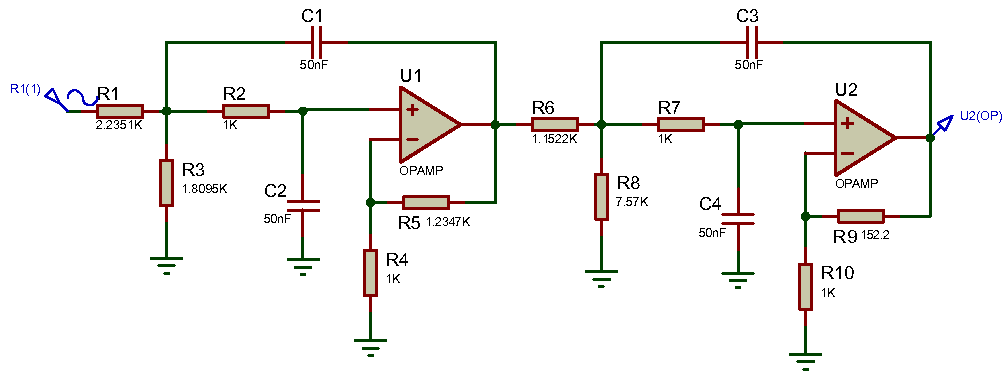
\includegraphics[width=\linewidth]{../Figures/ckt_d}
    \caption{Proteus circuit for fourth order lowpass filter designed in Problem 4}
    \label{fig:protD}
\end{figure}
\proteusObservationA{protD}{0}{3.177}{lowpass filter designed in Problem 4}
\mysub{Design of highpass filter using RC-CR transformation}
\problem{Apply RC-CR transformation in your filter circuit obtained in Problem 4, to obtain the highpass filter.}
RC-CR transformation is a technique used to convert lowpass filters to highpass filters, where each resistance is converted to a capacitor with capacitance $\ddfrac{1}{R}$ and each capacitor is converted to a resistance with value $\ddfrac{1}{C}$. Converting the normalized filter in Figure~\ref{fig:fourthorder} into an highpass filter using RC-CR transformation, we need to perform gain compensation (reduction) for both stages as,
\subsubsection*{Stage I}
\begin{equation}
    \begin{aligned}[b]
       &\frac{1}{s\times1}=Z_x||Z_y\\
       &\Rightarrow \frac{1}{s}=\ddfrac{\left(\frac{1}{sC_x}\right)\left(\frac{1}{sC_y}\right)}{\frac{1}{sC_x}+\frac{1}{sC_y}}\\
       &\Rightarrow \frac{1}{s}=\ddfrac{\frac{1}{s^2C_xC_y}}{\frac{C_x+C_y}{sCxC_y}}\\
       &\Rightarrow C_x+C_y=1
    \end{aligned}
    \label{eqn:cy-cx-parallel}
\end{equation}
Performing gain compensation as,
\begin{equation}
    \begin{aligned}[b]
        &\frac{Z_y}{Z_x+Z_y}=\frac{H}{K}=\frac{1}{2.2347}=0.4474\\
        &\Rightarrow 0.4474Z_x+0.4474Z_y=Z_y\\
        &\Rightarrow 0.5526Z_y=0.4474Z_x\\
        &\Rightarrow Z_y=0.8096 Z_x\\
        &\Rightarrow \frac{1}{sC_y}=0.8096 \frac{1}{sC_x}\\
        &\Rightarrow C_x=0.8096 C_y
    \end{aligned}
    \label{eqn:cy-cx-gain}
\end{equation}
Solving for $C_x$ and $C_y$ using Equation~\ref{eqn:cy-cx-parallel} and Equation~\ref{eqn:cy-cx-gain}, we get, $C_x=0.4474\text{ F}$ and $C_y=0.5526\text{ F}$.

\subsubsection*{Stage II}
\begin{equation}
    \begin{aligned}[b]
       &\frac{1}{s\times1}=Z_x'||Z_y'\\
       &\Rightarrow C_x'+C_y'=1
    \end{aligned}
    \label{eqn:cy-cx-parallel-i}
\end{equation}
Performing gain compensation as,
\begin{equation}
    \begin{aligned}[b]
        &\frac{Z_y'}{Z_x'+Z_y'}=\frac{H'}{K'}=\frac{1}{1.1522}=0.8679\\
        &\Rightarrow 0.8679Z_x'+0.8679Z_y'=Z_y'\\
        &\Rightarrow 0.1321Z_y'=0.8679Z_x'\\
        &\Rightarrow Z_y'=6.57 Z_x'\\
        &\Rightarrow \frac{1}{sC_y'}=6.57 \frac{1}{sC_x'}\\
        &\Rightarrow C_x'=6.57 C_y'
    \end{aligned}
    \label{eqn:cy-cx-gain-i}
\end{equation}
Solving for $C_x'$ and $C_y'$ using Equation~\ref{eqn:cy-cx-parallel-i} and Equation~\ref{eqn:cy-cx-gain-i}, we get, $C_x'=0.8679\text{ F}$ and $C_y=0.1321\text{ F}$.
\begin{figure}[H]
    \centering
    \figfourthorderhp
    \caption{Fourth order butterworth normalized highpass filter using RC-CR transformation}
    \label{fig:fourthorderhp}
\end{figure}
\mysub{Design of highpass filter at required half power frequency}
\problem{Finally obtain a highpass filter (from Figure~\ref{fig:fourthorderhp}) having half power frequency of 4.775 kHz with practically realizable elements. Realize the network and observe the response and note down the gain in passband and half power frequency.} \pagebreak
Here,
\begin{fleqn}[\parindent]
   \begin{equation*}
      \begin{split}
         &\text{Half power frequency of designed normalized filter } (\omega_o)=1 \text{ rad/s}\\
         &\text{Required half power frequency }(\Omega)=4.775 \text{ KHz} =2\pi\times4.775\times10^3 \text{ rad/s} \\
         &\text{Frequency scaling factor }(K_f)=\frac{\Omega}{\omega_o}=\frac{2\pi\times4.775\times10^3}{1}\approx 30\times10^3
         \end{split}
      \end{equation*}
\end{fleqn}
Since the values of resistance is unchanged with this scaling factor, let us use the magnitude scaling factor $K_m=10^3$ to make the values practically realizable. The scaled elemental values are,
\begin{equation*}
    \begin{aligned}
        &R_a=1\times10^3=1 \text{ K}\Omega \quad &&R_a'=1\times10^3=1 \text{ K}\Omega\\
        &R_b=1.2347\times10^3=1.2347 \text{ K}\Omega \quad &&R_b'=0.1522\times10^4=152.2 \text{ }\Omega\\
        &R_1=1\times10^3=1 \text{ K}\Omega \quad &&R_1'=1\times10^3=1 \text{ K}\Omega\\
        &R_2=1\times10^3=1 \text{ K}\Omega \quad &&R_2'=1\times10^3=1 \text{ K}\Omega\\
        &C_x= \ddfrac{0.4474}{10^3\times30\times10^3}=14.913\text{ nF}  \quad && 
        C_x'= \ddfrac{0.8679}{10^3\times30\times10^3}=28.93\text{ nF}  \\
        &C_y =\ddfrac{0.5526}{10^3\times30\times10^3}=18.42\text{ nF}  \quad && 
        C_y'= \ddfrac{0.1321}{10^3\times30\times10^3}=4.4\text{ nF}  \\
        &C_2 =\ddfrac{1}{10^3\times30\times10^3}=33.33\text{ nF}  \quad && 
        C_2'= \ddfrac{1}{10^3\times30\times10^3}=33.33\text{ nF}  \\
    \end{aligned}
\end{equation*}
\begin{figure}[H]
    \centering
    \figfourthorderhpfinal
    \caption{Fourth order butterworth highpass filter at half power frequency $4.775$ KHz}
    \label{fig:fourthorderhpfinal}
\end{figure}

\begin{figure}[H]
    \centering
    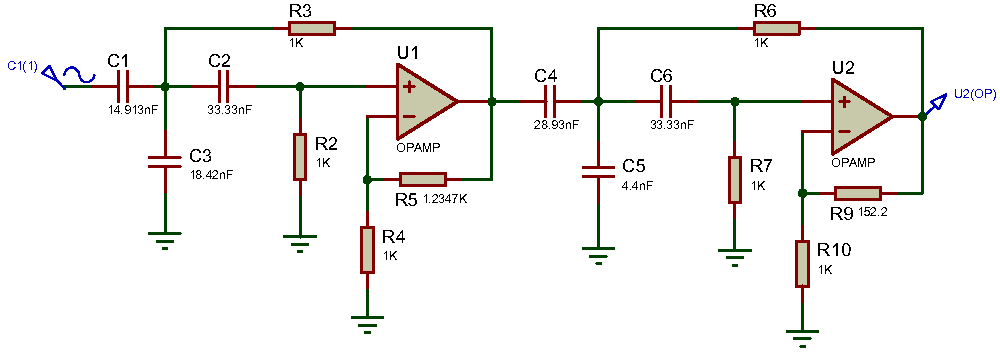
\includegraphics[width=\linewidth]{../Figures/ckt_f}
    \caption{Proteus circuit for fourth order highpass filter designed in Problem 6}
    \label{fig:protF}
\end{figure}
\proteusObservationA{protF}{0}{4.79}{highpass filter designed in Problem 6}
\section{Discussion and Conclusion}
In this lab experiment, we dealt with cascading of biquad circuits to design higher order filters using Sallen-Key biquad circuit shown in Figure~\ref{fig:ques}. The derivation for the transfer function of a Sallen-Key circuit was understood as a part of the experiment. Then using the transfer function, a set of design-rules can be established, out of which the report uses the default (equal element values) rule to calculate the elemental values for the different stages of the cascade network. Once the values are calculated, gain compensation (in the case of this lab report, gain reduction) was performed to get the desired gain. Once the normalized lowpass filter is obtained, it is scaled using the scaling formulae to get the desired response at required half power frequency. Next, RC-CR transformation is performed to convert the normalized lowpass filter to a normalized highpass filter. Once the normalized high pass filter is obtained, similar scaling is applied to get the desired response at desired half power frequency.\\
Hence, the objectives of the lab were fulfilled with the understanding of the mentioned topics.
    \end{document}